\documentclass[12pt, twoside]{article} 
\newcommand{\hdir}{.}
\usepackage{./jmlda}
%\usepackage[round]{natbib}
\usepackage[square,sort,comma,numbers]{natbib}
\usepackage{rotating}
\usepackage{tabularx} % for 'tabularx' env. and 'X' col. type
\setlength\extrarowheight{2pt} % make the tables look less cramped
\usepackage{hyperref}
\usepackage{graphics}
\usepackage{comment}
% теоремы
\newtheorem{theorem_takkens}{Таккенс \cite{takkens}}
\newtheorem{def_1}{Динамическая система}

\begin{document}
\title
	[Детекция зависимостей во временных рядах]
	{Детекция зависимостей во временных рядах}
\author
	[I. M. Latypov]
	{I. M. Latypov, E. Vladimirov, V. V. Strizhov}
\email
	{latypov.im@phystech.edu}
\organization	
	{MIPT}	
\abstract
	{
		Для многих прикладных задач, связанных с динамическими системами, требуется решать задачу выявления причинно-следственных зависимостей между временными рядами. 
		Выявление этих зависимостей может улучшить качество модели, или рассматриваться как отдельная задача классификации. 
		В данной работе для обнаружения подобных зависимостей предлагается использовать **модели пространства состояний**: скрытые состояния модели ODE-RNN рассматриваются 
		как представление временного ряда, и показывается что к этому представлению применим метод сходящегося перекрестного отображения (Convergent Cross Mapping).
		Работа метода проверяется на данных акселерометра и гироскопа при выполнении упражений.
		
	%	При прогнозировании временных рядов, зависящих от других временных рядов, требуется решить задачу выявления связей между ними.
	%	Предполагается, что добавление связанных временных рядов в прогностическую модель повысит качество прогноза. В данной работе для
	%	обнаружения зависимостей между временными рядами предлагается совместить Convergent Cross Mapping с ODE-RNN. 
		}
\bigskip
\noindent

\maketitle
\textbf{Ключевые слова}: \emph{Neural CDE, CCM, временные ряды}

\section{Введение}
		Работа посвящена задаче поиска причинно-следственных связей между временными рядами. Эта задача актуальна, поскольку на практике у изучаемой динамической системы несколько наблюдаемых величин \cite{dataset_mlru}, измерения которых представляют собой временной ряд. Исследование этих рядов является частью задачи исследования системы. Выявление причинно-следственных взаимосвязей между этими временными рядами наблюдаемых величин может рассматриваться как подзадача или как основная задача, например на основе анализа зависимости временных рядов данных гироскопов у танцующей пары можно делать выводы о качестве их взаимодействия.
		
		%	Наша цель - развить идею метода сходящегося перекрестного отображения. Изначально этот метод является непараметрическим, мы показываем что можно приме
		% Далее в разделе \hyperref[sec:math_form]{<<математическая постановка>>} привелена строгая постановка задачи и предлагаемый метод решения. В разделе \hyperref[sec:theor_background]{<<теоритичесие предпосылки>>} приведены теоритические предпосылки на которых основывается предлагаемый метод. 
		
\section{Связанные работы}	
\label{sec: related_works}
	
	Кросс Корреляция - метод проверяет коррреляцию временных рядов при из сдвигах. Зависимость оценивается на основе максимальной полученной корреляции.
	
	Тест Гренжера \cite{Seth2007} - обучается модель для предсказывания одного ряда. Обучается другая модель для предсказания второго ряда. Если качество предсказаний на второй модели существенно возрастает, то делается вывод о зависимости временных рядов.
	
	 Кластеризация квазипериодических временных рядов для распознавания человеческой деятельности \cite{Grabovoy2018} - использование метода главных компонент с новой метрикой, \cite{Kwapisz2010} - описывает метод построения описания объекта на основе экспертно определенных генерирующих функций.
	Метод перекрестного сходящегося отображения \cite{McCracken2014} будет рассмотрен далее в деталях как основа для построения нашего метода.
	
	Приведем достоинства и недостатки некоторых из них в таблице 1.

\begin{table}[]
	\begin{tabular}{|l|l|l|}
		\hline
		Метод                                                                  & достоинства                                                                                                 & недостатки                                                                                                                                                               \\ \hline
		Тест Грэнджера                                                         & Легко применять                                                                                             & \begin{tabular}[c]{@{}l@{}}Не дает представлений о виде \\ зависимости рядов. \\ Предсказания могут не \\ улучшиться из-за неверной модели.\end{tabular}                 \\ \hline
		Кросс Корреляция                                                       & Легко применять                                                                                             & \begin{tabular}[c]{@{}l@{}}Квадратичное от длины ряда \\ \\ время работы. \\ Корреляция не является достаточным \\ \\ условием зависимости\end{tabular}                  \\ \hline
		CCM                                                                    & \begin{tabular}[c]{@{}l@{}}Легко применять.\\  Работает лучше \\ методов предложенных \\ выше.\end{tabular} & \begin{tabular}[c]{@{}l@{}}Квадратичное от длины ряда время работы.\\ \\  Ислледование \textbackslash{}cite\{McCracken2014\} \\ выделяет другие недостатки.\end{tabular} \\ \hline
		\begin{tabular}[c]{@{}l@{}}CСM + ODE-RNN\\ (предлагаемый)\end{tabular} & \begin{tabular}[c]{@{}l@{}}Может работать с многомерными\\ временными рядами\end{tabular}                   & \begin{tabular}[c]{@{}l@{}}Нужно обучать\\ \\ Квадратичное от длины ряда время работы\end{tabular}                                                                       \\ \hline
	\end{tabular}
\end{table}
			
	
\section{Математическая постановка}
\label{sec:math_form}

Обозначим $T = \{t_1, ... t_k\}$ - моменты наблюдений. И введем обозначения 

$$\mathbf{x} = \{\mathbf{x_1}, \mathbf{x_2}, ... \mathbf{x_k}\} , \mathbf{y} = \{\mathbf{y_1}, \mathbf{y_2}, ... \mathbf{y_k}\}$$

  наблюдения за парой многомерных временных рядов. $x_i \in \mathbb R^m$, $y_i \in \mathbb R^n$,   в работе опыты проводятся при $m = n = 3$. Наблюдения $x_i, y_i$ сделаны в момент $t_i$. Промежутки между наблюдениями одинаковы, то есть частота семплирования рядов постоянна.

Ставится задача построения отображения $\phi : \{\mathbb{x} \times \mathbb{y}\} \rightarrow \mathbb{R}$ по значениям которой будет делаться вывод о зависимости временных рядов.

\section{предлагаемый метод}
	В качестве основы для модели берется метод сходящегося перекрестного отобраажения, поэтому рассмотрим его подробно. Метод применяется для пары одномерных временных рядов $\mathbf{x} = [x_1 , ..., x_N]$  и $\mathbf{y} = [y_1, ..., y_N]$. Индексирование такое же как в постановке.
	Идея метода основана не теореме Таккенса \cite{takkens}. Теорема утверждает, что для временного ряда, представляющего собой наблюдения за динамической системой и удовлетворяющего перечисленным выше условиям, по векторам $[x_i, x_{i+1}, ..., x_{L -1}]$ можно построить изоморфизм в прострванство, в котором развивается динамическая система. То есть такие вектора описывают динамическую систему. Здесь $L$ - размерность отображения, далее будем называть это размерностью погружения. Согласно теореме должно быть выполнено $L \geq 2m$, где $m$ - истинная размерность системы. Чаще всего $m$ нам не известно. 
	
	Метод рассматривает отображение временных рядов в траекторное подпространство с матрицей Ганкеля временного ряда и оценивает, насколько хорошо траектория эволюции одного ряда восставнавливается по траекторий эволюций другого. Опишем как это делается. По рядам строится матрица Ганкеля:
	
	$$
	\mathbf{H}_{x} =
	\left( {\begin{array}{ccccc}
			x_1 & x_2 & ... & x_{L-1} & x_L\\
			x_2 & x_3 & ... & x_{L} & x_{L +1}\\
			... & ... & ... & ...   & ... \\
			x_{N-L+1} & x_{N-L +2} & ... & x_{N-1} & x_N\\
	\end{array} } \right)
	$$
	
	$L$ - размерность погружения, используемая для построения отображения в пространство эводюции системы. Так же строится матрица Ганкеля второго ряда $\mathbf{H}_y$.
	Обозначим через $\mathbf{x}_{t+L -1}$ $t$-ую строку $H_x$, $\mathbf{y}_{t+L -1}$ $t$-ую строку $H_y$. Тогда вектора $\mathbf{x}_t$ рассматриваются как точки в траекторнорм пространстве $\mathbf{M}_x$, $\mathbf{н}_t$ - как точки в траекторнорм пространстве $\mathbf{M}_y$. В этих пространствах выбирается евклидова метрика.
	Для восстановления измерения $y$ в момент времени $t\in L,..., N$ найдем $k$ ближайших соседей вектора $\mathbf{x}_t$. Обозначим их по возрастанию расстояния до $\mathbf{x}_t$:
	
	$$\mathbf{x}_{t_1}, \mathbf{x}_{t_2}, ...,\mathbf{x}_{t_k}$$. 
	
	После этого строится прогноз $y_t$ следующим образом:
	
	$$
	y^t = \sum^k_{i = 1}w_iy_{t_i}$$
		$$	w_i = \frac{u^i}{\sum_i u_i}, \qquad u_i = \exp(-\frac{\|x_t - x_{t_i}\|_2}{\|x_t - x_{t_k}с\|_2})
	$$
	
	Для обнаружения зависимости рядов рассматривается корреляция между предсказаниями и значениями ряда. На основании величины корреляции делается вывод о зависимости или независимости рядов.
	
	Чтобы развить этот метод рассмотрим параметрическое построение погружений. Для этого обратимся к моделям пространства состояний -- моделям дискретного описания динамической системы. При таком подходе совсместно с временным рядом рассматривается дополнительный вектор скрытых состояний, который эволюционирует совместно с наблюдениями за системой.
	
	В самом простом виде уравнения развития скрытых состояний системы могут выглядеть следующим образом: вектор скрытых состояний системы $u$, вектор наблюдений за системой $x$

\begin{equation}
	\begin{split}
		u_t = F(u_{t-1}, y_t) \\ 
		z_{t} = G(u_t, y_t)
	\end{split}
\end{equation}

$z$ здесь моделируемая величина. Второе уравнение нам не нужно, так что далее рассматриваем только первое, из которого получаются скрытые состояния.

Итоговая модель выглядит крайне просто:

\begin{equation}
	\begin{split}
		u_0 = f(x_0) \\ 
		u_{k + 1} = \psi(u_k, x_k)
	\end{split}
\end{equation}

Мы выделили два принципиально различных способа задания функции $\psi$ -- непрерывное и дискретное и рассмотрели их в экспериментах. Дискретное изменение моделирорвалось с помощью GRU модуля. Для моделирования непрерывных изменений была взята модель ODE-RNN \cite{rubanova2019latent}.



---------------------------------------------------------------------------

возможно понадобится краткое описание ODE-RNN

---------------------------------------------------------------------------

\section{анализ свойств предложенного метода}
\label{sec:theor_background}
---------------------------------------------------------------------------

Предлагаю вообще убрать этот раздел

---------------------------------------------------------------------------


\begin{comment}
---------------------------------------------------------------------------
это все убрать поскольку уже рассказано в описании CCM
---------------------------------------------------------------------------
Основой для построения метода послужила теорема Таккенса и метод CCM основанный на ней.


Пусть $M$ - компактное многообразие размерности $m$

\begin{def_1}
	динамической системой $\phi$ c дискретным временем на $M$ назовем диффеоморфизм $\phi: M\rightarrow M$. 
	
	Эволюция системы начинается с $x_0 \in M$ и следующие состояния определятся рекурсивно $x_{t+ 1} = \phi(x_t)$. 
\end{def_1}

пусть $\phi$ -динамическая система. Определим гладкую функцию $y: M \rightarrow \mathbb{R}$ - наблюдения за динамической системой. Хочется из набора наблюдений получить информацию об эволюции системы $\phi$ в $M$.

Для этого нам понадобится следующая теорема

\begin{theorem_takkens}
Пусть $M$ - компактное многообразие размерности $m$. Для пар $(\phi, y)$, где $\phi : M \rightarrow M$ гладкий диффеоморфизм и $y: M \rightarrow \mathbb R$ гладкая функция,
 общим свойством является то, что $\Phi: M \rightarrow \mathbb R^{2m + 1}$, определяемое как 

$$\Phi_{(\phi. y)} (x) = (y(x), y \circ \phi(x), ... , y \circ \phi^{2m}(x)) $$
является вложением $A(\phi) \rightarrow \mathbb R^{2m + 1}$. Под гладкостью понимается дважды непрерывная дифференцируемость.
\end{theorem_takkens}

$A(\phi)$ - аттрактор динамической системы.

То есть для изучения свойств траектории динамической системы $phi$ можно использовать траектории, которые получаются при этих погружениях.

Пусть даны две динамические системы: $\phi$ с наблюдениями $x$ на многообразии $M_x$ и $\psi$  c наблюдениями $y$ на многообразии $M_y$. 
Нужно выяснить, есть ли причинно-следственная связь между системами. Поскольку мы не имеем представления об устройстве многообразий рассмотрим их вложения $\Phi_(\phi, x)$ и $\Phi_(\psi, y)$.

(TODO   расписать здесь идею CCM) 

Мы хотим проверить, можно ли вместо таких погружений рассматривать систему $psi$, которая будет развиваться в зависимости от наблюдений за $\phi$. Более формально:

Есть динамическая система $\phi$, которая развивается в многообразии $M$ размерности $m$. $y: M \rightarrow \mathbb R$ - непрерывный наблюдатель за системой $\phi$.
Введем (динамическую сисему ?) $\psi: \mathbb R^{n + 1} \rightarrow \mathbb {R}$. Её вектора обозначим $\gamma$ так, что 

\begin{equation}
	\begin{split}
		\gamma_0 = f(y_0) \\ 
		\gamma_{k + 1} = \psi(\gamma_k, y_k)
    \end{split}
\end{equation}

Если динамическая система $\phi$ задана с непрерывным временем, то вместо функции $\psi$ рассмотрим интеграл

\begin{equation}
	\begin{split}
		\gamma(t_0) = f(y(t_0)) \\
		\gamma(t) = \int_{t_0}^{t} \psi(\gamma(\tau), y(\tau)) d\tau
    \end{split}
\end{equation}

Ввиду невозможности непрерывного измерения $y$ при интегрировании будем использовать интерполяцию или $ y(\tau) = g(\gamma(t))$ и уточнять y по мере интегрирования.

\end{comment}


\section{Эксперименты}
\label{experiments}
	Кратко опишем выбрку на которой проводились эксперименты. Данные представляют собой записи показаний акселерометра и гироскопа при ходьбе и при беге на протяжении 30 - 40 секунд. За это время делается примерно 15 движений. Частота семплирования равна 200 Гц. Датчики находятся на концах рук, так что можем рассматривать пары временных рядов и применять к ним метод. Можно посмотреть пример временного ряда гироскопа на картинке \ref{ряд}
	
\begin{figure}
	\centering
	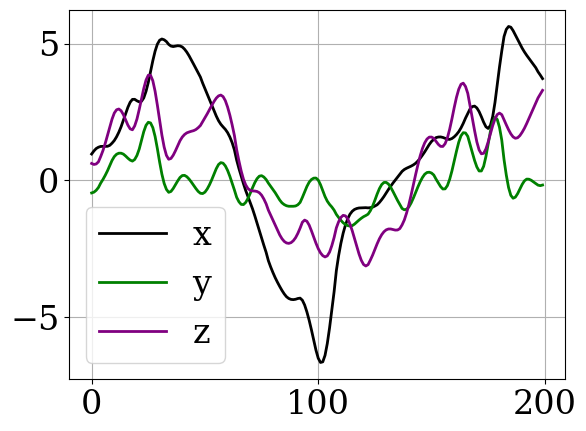
\includegraphics[scale=0.75]{images/ряд.jpg} 
	\caption{Ряд значений показаний гироскопа на отрезке в 250 семплов \label{ряд}}
\end{figure}


	Сначала рассмотрим работу метода на паре одномерных временных рядов. В качестве функции $\psi$ используется ODE-RNN.
	Рассмортим траектории временных рядов в скрытых состояниях. Для этого в методе CCM берется матрица ганкеля и из него выделяются главные компоненты. Подробнее в работе \cite{Usmanova2018}.  
	получившиеся траектории можно увидеть на картинках \ref{trajectory}. Для наглядности траектории были спроецированы на сферу.
	
\begin{figure}
	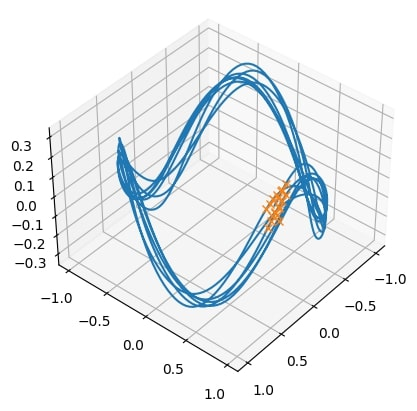
\includegraphics[width = 0.5\textwidth]{images/trajectory_CCM.jpg} \hfill
	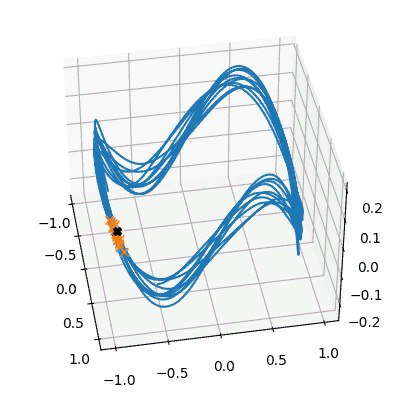
\includegraphics[width = 0.5\textwidth]{images/trajectory_CCM_right.jpg}
	\caption{слева направо - траектория скрытых состояний при использовании CCM левого/правого гироскопа\label{trajectory}}
\end{figure}
	
	В нашем методе матрица скрытых состояний получается не ганкелевой, поэтому к ней перед построением траекторий применяется метод многомерной гусеницы (анализ сингулярного спектра) \cite{SSA1997}


\begin{figure}
	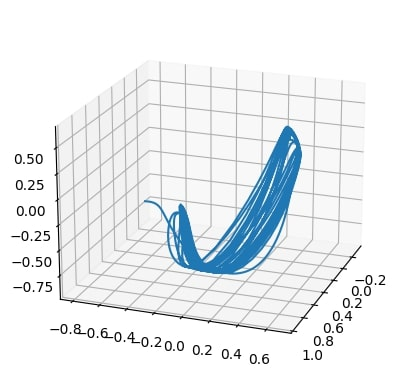
\includegraphics[width = 0.5\textwidth]{images/trajectory_left.jpg} \hfill
	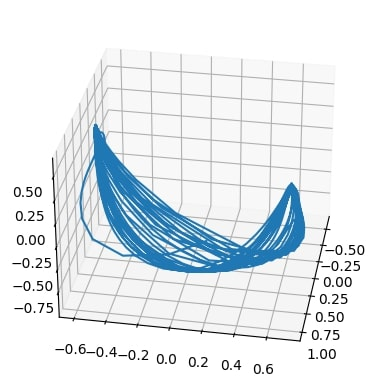
\includegraphics[width = 0.5\textwidth]{images/trajectory_right.jpg}
	\caption{слева направо - траектория скрытых состояний при использовании ODE-RNN + гусеница левого/правого гироскопа}
\end{figure}		
	
	То есть в скрытых состояниях появляются одинаковые периодические структуры, поэтому можем применить метод CCM  скрытым состояниям. Результат применения можно увидеть на графиках \label{CCM_apply}. Для сравнения приведен результат применения методов к паре гироскоп - рандомная последовательность.
	
---------------------------------------------------------------

нужно будет поменять label в графиках
	
---------------------------------------------------------------

\begin{figure}
	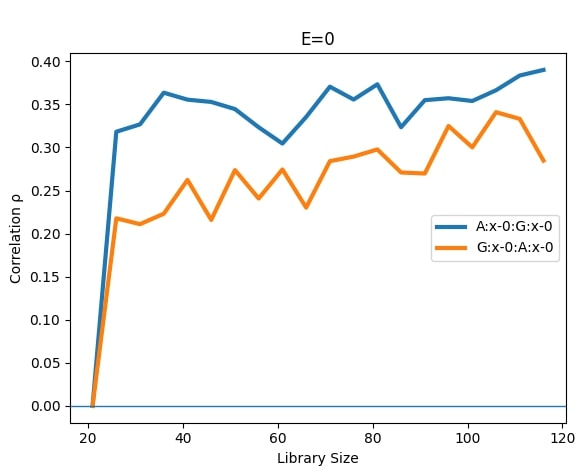
\includegraphics[width = 0.5\textwidth]{images/CCM_experiments/A_x-G_x.jpg} \hfill
	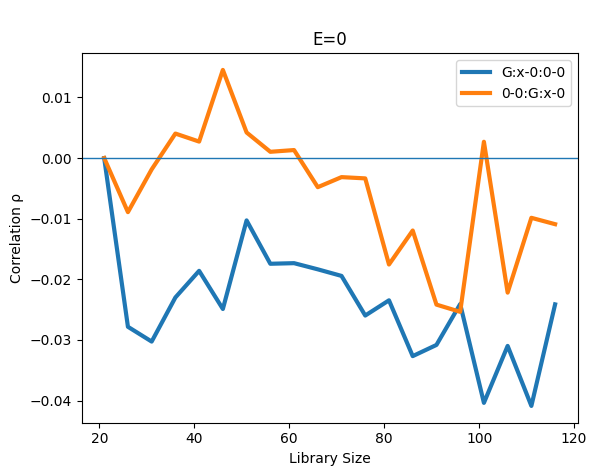
\includegraphics[width = 0.5\textwidth]{images/CCM_experiments/A_x-R_0.jpg} 
	\\[\smallskipamount]
	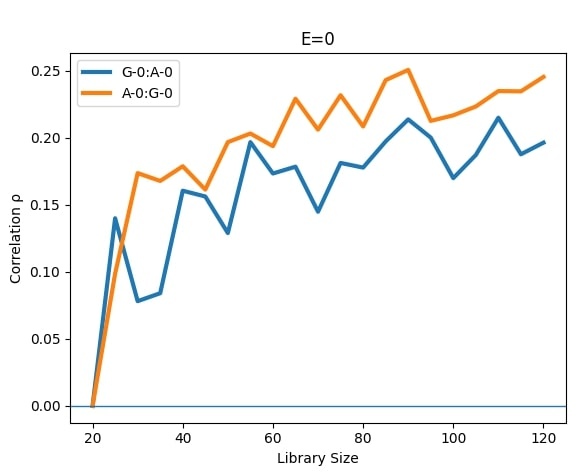
\includegraphics[width = 0.5\textwidth]{images/ODE_RNN_experiments/A_0-G_0.jpg} \hfill
	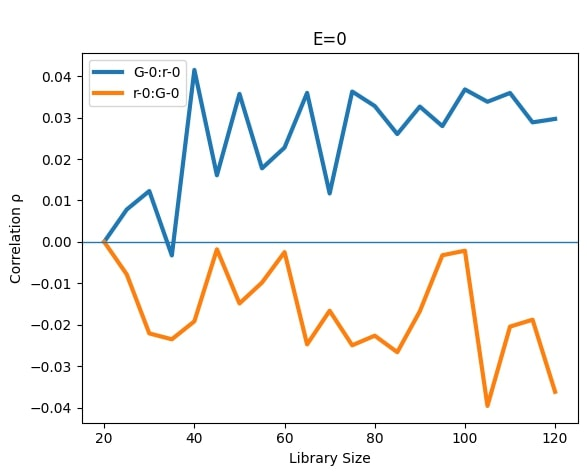
\includegraphics[width = 0.5\textwidth]{images/ODE_RNN_experiments/A_0-R_0.jpg} 
	\caption{слева направо, сверху вниз: CCM акселерометр - гироскоп, CCM акселерометр - random, ODE-RNN акселерометр - гироскоп, ODE-RNN акселерометр - random \label{CCM_apply}}
\end{figure}

Видно что предлагаемый метод может выделять зависимость и независимость на рассмотренных данных так же как   CCM.

Но это не единственная возможность метода. Как отмечалось ранее - наблюдения на датасете с акселерометром - трехмерные.

----------------------------------------------------------------

красивые картинки про эксперименты с трехмерными данными. Не совсем понимаю что поставить

----------------------------------------------------------------

\section{Заключение}

Предложили метод для выявления взаимной зависимости временных рядов. Опыты показали что он работает на паре измерений двух датчиков на теле. В отличие от своих аналогов он позволяет работать с многомерными временными рядами. Границы применимости метода --- пока открытый вопрос.


\section{Список литературы}
\bibliographystyle{plain}
\bibliography{library.bib}

\end{document}